\section{问题三：客户分层与差异化挽留策略}

在问题二确定逻辑回归模型并完成 SHAP 归因分析后，
本节将模型输出的流失概率转化为可操作的客户分层方案，
使运营商能够依据不同层级客户的特征差异，配置有限的挽留资源。

\subsection{客户流失风险分层}

分层需解决两个问题：怎么划分层级，以及划分出的层级是否在业务上
有区隔意义。本文采用分位数切分法，以模型输出的全量预测概率为
依据：中位数（P50 = 0.373）以下为低风险，P50 至 P80（0.770）
之间为中风险，P80 以上为高风险。之所以选择 P50/P80 而非等距
切分（如 0-0.33/0.33-0.66/0.66-1），是因为预测概率分布呈现
明显的右偏形态（偏度约为 0.59），大部分客户集中在低概率区间；
采用等距切分将导致中、高风险层级过于稀疏，不利于后续制定
有统计意义的差异化策略。

按上述标准，高风险客户 1409 人（20.0\%），中风险客户 2112 人
（30.0\%），低风险客户 3522 人（50.0\%），如图 \ref{fig:risk_tiers}
所示。

\begin{figure}[H]
    \centering
    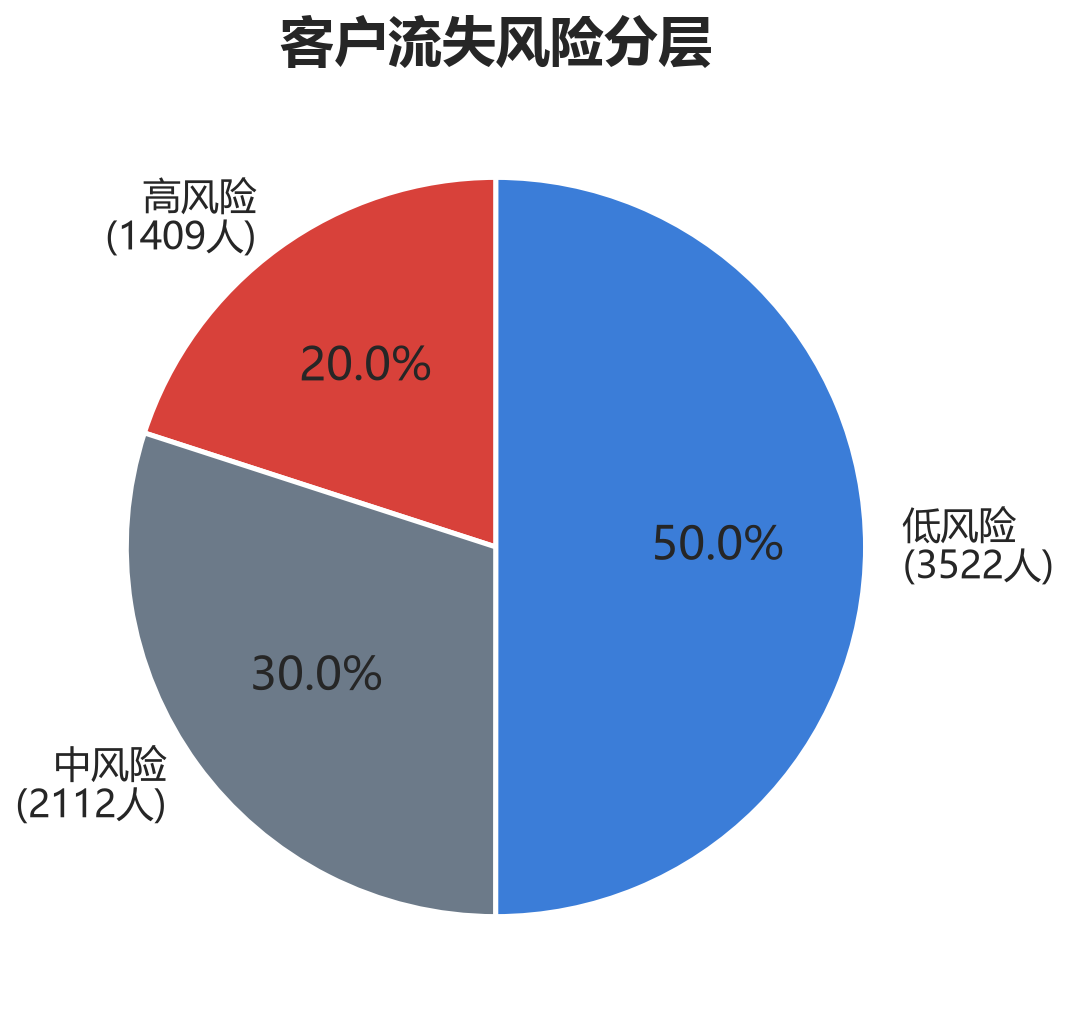
\includegraphics[width=0.5\textwidth]{figures/risk_tiers.png}
    \caption{客户流失风险分层}
    \label{fig:risk_tiers}
\end{figure}

为检验分层在实际业务中的区分度，选取在网时长、月消费金额、
CLTV、月付合同比例、光纤比例和有家属比例六个维度，
计算各层级的均值/占比，如表 \ref{tab:tier_comparison} 所示。

\begin{table}[H]
    \centering
    \caption{各风险层级特征对比}
    \label{tab:tier_comparison}
    \small
    \begin{tabular}{lccc}
        \toprule
        指标 & 低风险 & 中风险 & 高风险 \\
        \midrule
        人数 & 3522 & 2112 & 1409 \\
        占比 & 50.0\% & 30.0\% & 20.0\% \\
        在网时长（月） & 46.0 & 23.8 & 11.1 \\
        月消费金额（美元） & 57.1 & 66.8 & 80.8 \\
        CLTV（美元） & 4634 & 4271 & 4009 \\
        光纤比例 & 22.9\% & 49.0\% & 88.9\% \\
        月付合同比例 & 19.5\% & 84.3\% & 99.9\% \\
        有家属比例 & 41.5\% & 7.9\% & 0.0\% \\
        \bottomrule
    \end{tabular}
\end{table}

各层级在表 \ref{tab:tier_comparison} 的六个维度上均形成了清晰的
梯度。从低风险到高风险，在网时长从 46 个月降至 11 个月，月付
合同占比从 19.5\% 陡升至 99.9\%，有家属比例从 41.5\% 降为 0——
这三项特征的层级间落差与问题一中 EDA 发现的"新客户 + 月付 +
无家庭绑定是最优流失信号"完全吻合。光纤比例从低风险的 22.9\%
上升到高风险的 88.9\%，与问题二 SHAP 排序中光纤服务位居 Top 3
的结论一致。CLTV 随风险升高而降低（4634 → 4009 美元），但降幅
相对温和，说明仅凭 CLTV 的绝对值不足以区分风险高低，必须结合
合同形式与在网状态等行为特征才能准确判断。

值得单独指出的是，高风险层的月付合同比例达 99.9\% 且无任何客户
有家属，这呼应了问题二的分析结论——合同期限和家庭绑定是最有
效的两道"防流失壁垒"，缺乏这两道壁垒的客户几乎全部落入了
高风险组。

\subsection{差异化挽留策略}

分层的目的不是贴标签，而是为不同特征构成的客户群匹配不同成本
和力度的干预手段。基于表 \ref{tab:tier_comparison} 的层级画像
和问题二的 Top 5 关键因子，本文提出以下分层方案。

\begin{enumerate}
    \item \textbf{高风险客户。}
    该群体在网不足一年、几乎全部按月付费、无家庭绑定、
    近九成使用光纤——七成以上的高风险客户同时满足这四类属性。
    对他们而言，离网几乎没有合同或家庭的约束，
    只要竞争对手提供稍低的价格就可能触发流失。
    针对这一特征，挽留的核心是制造"留下来的理由"，
    措施包括：推送年付合同折扣（首年 7 折），
    将客户从随时可退的月付模式中拉入有退出成本的年付合约；
    对光纤用户叠加免费提速或安全防护等增值权益，
    弥补价格敏感群体对高月费的不满。
    这一层是挽留资源投入的绝对重点，其人口规模虽仅占 20\%，
    但流失概率最高，单位挽留投入的预期回报也最大。

    \item \textbf{中风险客户。}
    该群体流失概率居中，从表 \ref{tab:tier_comparison} 可以看出
    他们处于"灰色地带"——部分客户已有一定在网时长
    （均值 23.8 个月），但仍有 84.3\% 停留在月付模式。
    这说明中风险层的核心矛盾并非对服务本身的不满，
    而是尚未被引导进入长期合同。
    对此层的策略应以转化而非防御为主：对光纤客户提供带宽升级
    或流媒体会员权益，增加服务吸引力；对月付客户推荐年付转化
    优惠，借助已有的在网时长基础推动其完成从月付到年付的跃迁，
    从而自然降低未来的流失风险。

    \item \textbf{低风险客户。}
    该群体在网普遍超过三年、年付或两年合同为主、
    四成以上有家庭绑定，流失概率在各层级中最低。
    他们不需要激进的挽留手段——过度推送反而可能引起反感。
    维持策略集中于合同到期前的续约提醒与小幅优惠，
    以最低的干预成本保持现有的客户粘性。
\end{enumerate}

\subsection{预期收益与成本分析}

挽留策略的实际价值最终取决于投入产出比。
本节以高风险客户为干预对象进行保守估算，
假设三个关键参数：
（1）触达率为 60\%——考虑到电话外呼、邮件和 APP 推送的
叠加覆盖能力，实际触达比例通常高于此数；
（2）挽留成功率为 30\%——基于年付折扣在类似电信营销活动中
的历史参考数据；
（3）人均挽留成本为 50 美元——涵盖首年折扣让利和运营费用。

在上述假设下，各中间结果与最终的投入产出核算见表 \ref{tab:roi}。

\begin{table}[H]
    \centering
    \caption{挽留策略投入产出估算}
    \label{tab:roi}
    \small
    \begin{tabular}{lrl}
        \toprule
        指标 & 数值 & 说明 \\
        \midrule
        高风险客户数 & 1409 人 & 占总客户 20\% \\
        预期触达率 & 60\% & 多渠道覆盖比例 \\
        预期挽留率 & 30\% & 触达客户中的转化比例 \\
        预期挽回人数 & 254 人 & $1409 \times 0.6 \times 0.3$ \\
        平均 CLTV & \$4400 & 全量客户均值 \\
        预期挽回收益 & \$1,116,003 & $254 \times 4400$ \\
        挽留总成本 & \$42,270 & 触达人数 $\times$ 人均 \$50 \\
        \textbf{投资回报率} & \textbf{25.4 倍} & （收益 $-$ 成本） ÷ 成本 \\
        \bottomrule
    \end{tabular}
\end{table}

即在当前参数假设下，每投入 1 美元可获得约 25.4 美元的预期回报，
净收益约 107 万美元。
即使将触达率和挽留率各打对折（30\% 和 15\%），
ROI 仍保持在 6 倍以上，方案在经济层面具有较宽的容错空间。
